\documentclass{ximera}


\outcome{Understand the relationship between the graph of a function
  and the graph of its derivative.}  

\outcome{Understand the
  relationship between differentiability and continuity.}
\outcome{Understand secant lines and tangent lines.}

\outcome{Understand the definition of the derivative at a point.}

\outcome{Graph the derivative function.}

\outcome{Determine whether a piecewise function is differentiable.}


\title{Working with derivatives}

\begin{document}

\begin{abstract}
  Let's get some basic ideas related to derivatives under our belt.
\end{abstract}
\maketitle

Derivatives tell us information about functions. Given a function
$f(x)$, the slope of the tangent line tells us whether the function is
increasing (as $x$ increases) or decreasing (as $x$ increases).
In particular, if the function is increasing, then the derivative of the function is positive. If the function is decreasing, then the derivative of the function is negative. Let's put these facts to use:

\begin{question}
If $f'(x)$ is positive for all $x$ with $0\le x\le 1$, then which is
larger: $f(0)$ or $f(1)$?
    \begin{multipleChoice}
      \choice[correct]{$f(1)$}
      \choice{$f(0)$}
      \choice{Impossible to say with the information given.}
    \end{multipleChoice}  
\end{question}



\begin{question} 
If the line $y = 7x-4$ is tangent to $f(x)$ at $x=2$, find $f(2)$ and
$f'(2)$.
\begin{hint}
How is the derivative related to the plot of a function?
\end{hint}
\begin{multipleChoice}
\choice[correct]{$f(2) = 10$ and $f'(2) = 7$}
\choice{$f(2) = 3$, and $f'(2) = -4$}
\choice{$f(2) = 7x-4$, and $f'(2) = 7$}
\choice{$f(2) = 7x-4$, and $f'(2) = -4$}
\end{multipleChoice}
\end{question}


\begin{question}
Consider the following plot of a function $f(x)$:
\begin{image}
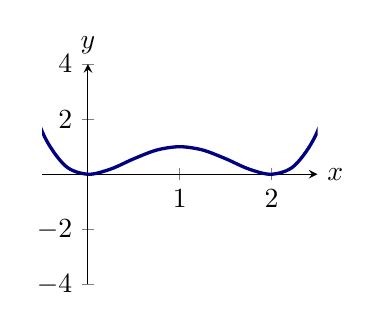
\begin{tikzpicture}
  \colorlet{penColor}{blue!50!black}
  \begin{axis}[
      domain=-3:3,
      width=2in,
      ymax=4,
      ymin=-4,
      %samples=100,
      axis lines =middle, xlabel=$x$, ylabel=$y$,
      every axis y label/.style={at=(current axis.above origin),anchor=south},
      every axis x label/.style={at=(current axis.right of origin),anchor=west}
    ]
    \addplot [very thick, penColor, smooth,domain=(-3:3)] {x^4-4*x^3+4*x^2};
  \end{axis}
\end{tikzpicture} 
\end{image}
Which of the following is a plot of the derivative of this function?
\begin{description}
\item[$p(x)$]
\begin{image}
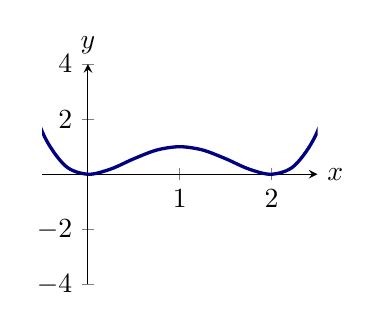
\begin{tikzpicture}
  \colorlet{penColor}{blue!50!black}
  \begin{axis}[
      domain=-3:3,
      width=2in,
      ymax=4,
      ymin=-4,
      %samples=100,
      axis lines =middle, xlabel=$x$, ylabel=$y$,
      every axis y label/.style={at=(current axis.above origin),anchor=south},
      every axis x label/.style={at=(current axis.right of origin),anchor=west}
    ]
    \addplot [very thick, penColor, smooth,domain=(-3:3)] {x^4-4*x^3+4*x^2};
  \end{axis}
\end{tikzpicture}
\end{image}

\item[$q(x)$]
\begin{image}
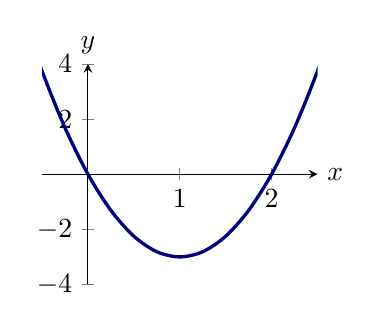
\begin{tikzpicture}
  \colorlet{penColor}{blue!50!black}
  \begin{axis}[
      domain=-3:3,
      width=2in,
      ymax=4,
      ymin=-4,
      %samples=100,
      axis lines =middle, xlabel=$x$, ylabel=$y$,
      every axis y label/.style={at=(current axis.above origin),anchor=south},
      every axis x label/.style={at=(current axis.right of origin),anchor=west}
    ]
    \addplot [very thick, penColor, smooth,domain=(-3:3)] {3*x^2-6*x};
  \end{axis}
\end{tikzpicture}
\end{image}

\item[$r(x)$]
\begin{image} 
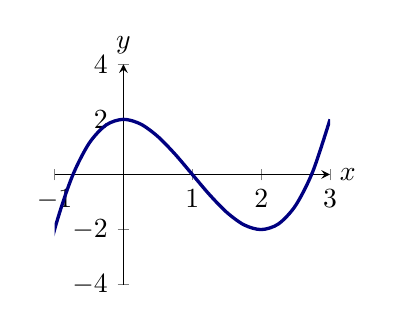
\begin{tikzpicture}
  \colorlet{penColor}{blue!50!black}  
  \begin{axis}[
      domain=-3:3,
      width=2in,
      ymax=4,
      ymin=-4,
      %samples=100,
      axis lines =middle, xlabel=$x$, ylabel=$y$,
      every axis y label/.style={at=(current axis.above origin),anchor=south},
      every axis x label/.style={at=(current axis.right of origin),anchor=west}
    ]
    \addplot [very thick, penColor, smooth,domain=(-3:3)] {x^3-3*x^2+2};
  \end{axis}
\end{tikzpicture}
\end{image}

\item[$s(x)$]
\begin{image} 
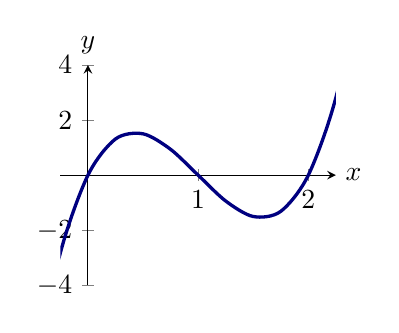
\begin{tikzpicture}
  \colorlet{penColor}{blue!50!black}
  \begin{axis}[
      domain=-3:3,
      width=2in,
      ymax=4,
      ymin=-4,
      %samples=100,
      axis lines =middle, xlabel=$x$, ylabel=$y$,
      every axis y label/.style={at=(current axis.above origin),anchor=south},
      every axis x label/.style={at=(current axis.right of origin),anchor=west}
    ]
    \addplot [very thick, penColor, smooth,domain=(-3:3)] {4*x^3-12*x^2 + 8*x};
  \end{axis}
\end{tikzpicture}
\end{image}
\begin{hint}
When the function is increasing (as $x$ increases), what can you say
about the derivative? When the function is decreasing (as $x$
increases), what can you say about the derivative?
\end{hint}
\begin{multipleChoice}
\choice[correct]{$f'(x) = s(x)$.}
\choice{$f'(x) = p(x)$}
\choice{$f'(x) = q(x)$}
\choice{$f'(x) = r(x)$}
\end{multipleChoice}
\end{question}


\begin{question}
Consider the following plot of a function $g(x)$:
\begin{image}
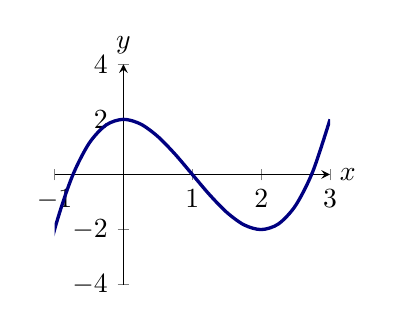
\begin{tikzpicture}
  \colorlet{penColor}{blue!50!black}  
  \begin{axis}[
      domain=-3:3,
      width=2in,
      ymax=4,
      ymin=-4,
      %samples=100,
      axis lines =middle, xlabel=$x$, ylabel=$y$,
      every axis y label/.style={at=(current axis.above origin),anchor=south},
      every axis x label/.style={at=(current axis.right of origin),anchor=west}
    ]
    \addplot [very thick, penColor, smooth,domain=(-3:3)] {x^3-3*x^2+2};
  \end{axis}
\end{tikzpicture}
\end{image}
Which of the following is a plot of the derivative of this function?
\begin{image}
\begin{array}{cccc}
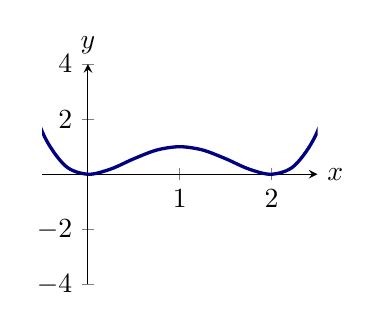
\begin{tikzpicture}
  \colorlet{penColor}{blue!50!black}
  \begin{axis}[
      domain=-3:3,
      width=2in,
      ymax=4,
      ymin=-4,
      %samples=100,
      axis lines =middle, xlabel=$x$, ylabel=$y$,
      every axis y label/.style={at=(current axis.above origin),anchor=south},
      every axis x label/.style={at=(current axis.right of origin),anchor=west}
    ]
    \addplot [very thick, penColor, smooth,domain=(-3:3)] {x^4-4*x^3+4*x^2};
  \end{axis}
\end{tikzpicture} & 
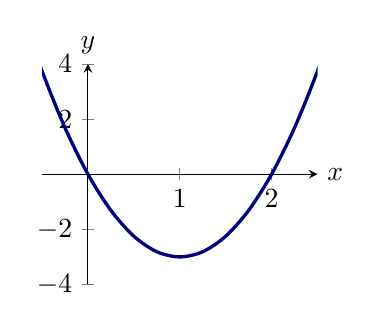
\begin{tikzpicture}
  \colorlet{penColor}{blue!50!black}
  \begin{axis}[
      domain=-3:3,
      width=2in,
      ymax=4,
      ymin=-4,
      %samples=100,
      axis lines =middle, xlabel=$x$, ylabel=$y$,
      every axis y label/.style={at=(current axis.above origin),anchor=south},
      every axis x label/.style={at=(current axis.right of origin),anchor=west}
    ]
    \addplot [very thick, penColor, smooth,domain=(-3:3)] {3*x^2-6*x};
  \end{axis}
\end{tikzpicture} & 
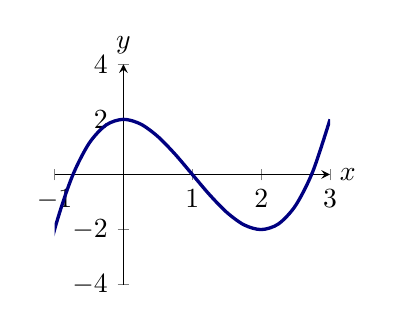
\begin{tikzpicture}
  \colorlet{penColor}{blue!50!black}  
  \begin{axis}[
      domain=-3:3,
      width=2in,
      ymax=4,
      ymin=-4,
      %samples=100,
      axis lines =middle, xlabel=$x$, ylabel=$y$,
      every axis y label/.style={at=(current axis.above origin),anchor=south},
      every axis x label/.style={at=(current axis.right of origin),anchor=west}
    ]
    \addplot [very thick, penColor, smooth,domain=(-3:3)] {x^3-3*x^2+2};
  \end{axis}
\end{tikzpicture} & 
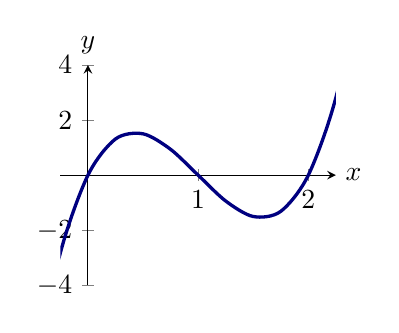
\begin{tikzpicture}
  \colorlet{penColor}{blue!50!black}
  \begin{axis}[
      domain=-3:3,
      width=2in,
      ymax=4,
      ymin=-4,
      %samples=100,
      axis lines =middle, xlabel=$x$, ylabel=$y$,
      every axis y label/.style={at=(current axis.above origin),anchor=south},
      every axis x label/.style={at=(current axis.right of origin),anchor=west}
    ]
    \addplot [very thick, penColor, smooth,domain=(-3:3)] {4*x^3-12*x^2 + 8*x};
  \end{axis}
\end{tikzpicture} \\
p(x) & q(x) & r(x) & s(x)
\end{array}
\end{image}
\begin{hint}
When the function is increasing (as $x$ increases), what can you say
about the derivative? When the function is decreasing (as $x$
increases), what can you say about the derivative?
\end{hint}
\begin{multipleChoice}
\choice[correct]{$g'(x) = q(x)$.}
\choice{$g'(x) = p(x)$}
\choice{$g'(x) = s(x)$}
\choice{$g'(x) = r(x)$}
\end{multipleChoice}
\end{question}




\begin{question}
Write down at least \textbf{five} questions for this lecture. After
you have your questions, label them as ``Level 1,'' ``Level 2,'' or ``Level 3'' where:
\begin{description}
\item[Level 1] Means you know the answer, or know exactly how to do this problem.
\item[Level 2] Means you think you know how to do the problem, or will soon learn how to do the problem.
\item[Level 3] Means you have no idea how to do the problem. 
\end{description}
  \begin{freeResponse}
  \end{freeResponse}
\end{question}

\end{document}
